\documentclass[10pt]{article}
\usepackage{multicol}
\usepackage{tcolorbox}
\usepackage{minted}
\usepackage{listings}
\usepackage{geometry}
\usepackage{titlesec}
\usepackage{amsmath}


\geometry{margin=13pt}
\pagestyle{empty}
\titlespacing*{\subsubsection}{0pt}{4pt}{2pt}
\tcbset{before skip=2pt, after skip=2pt, boxsep=0pt, halign=center}
\tcbset{left=2pt, right=2pt, top=2pt, bottom=2pt, lefttitle=5pt}
\tcbset{colback=white, colframe=black}
\newcommand{\code}[1]{\mintinline{text}{#1}}

% multicol parameters
\setlength{\premulticols}{2pt}
\setlength{\postmulticols}{2pt}
\setlength{\multicolsep}{2pt}
\setlength{\columnsep}{5pt}
\setlength{\parskip}{0pt}

\begin{document}
\begin{multicols*}{2}
    \subsubsection*{Computer Structure and Evolution}
    \begin{tcolorbox}[title=Internal Structure of Computer and CPU, halign=flush left]
        \tiny
        CPU: Controls the operation of the computer and performs arithmetic and logic operations.
        Memory: Stores data and instructions for the CPU.
        I/O: Transfer data between computer and external environment.
        System Bus: Connects the CPU, memory, and I/O devices, allowing them to communicate with each other.
        Control Unit: controls the operation of the CPU.
        ALU: performs data processing functions.
        Registers: provides storage internal to the CPU.
        CPU Bus: provides for communication among the control unit, ALU and registers.
    \end{tcolorbox}

    \begin{tcolorbox}[title=Benchmark]
        \begin{tabular}{ll}
            Clock Speed & pulse freq produced by clock (unit: Hz)                             \\
            Inst Count  & instruction count $I_c = \sum_i I_i$                                \\
            CPI         & average clocks per instruction $\sum_i \text{CPI} \times I_i / I_c$ \\
            Time        & processor time $T = \text{CPI} \times I_c/f$                        \\
            MIPS        & million instruction per second $f / (\text{CPI} \times 10^6)$       \\
            MFLOPS      & floating point operation $f / (\text{CPI} \times 10^6)$             \\
            SPEC        & standard performance evaluation corporation                         \\
        \end{tabular}
    \end{tcolorbox}

    \subsubsection*{Number Representation}
    \begin{tcolorbox}[title=2's Complement]
        \begin{tabular}{ll}
            range          & $-2^{n-1}$ to $2^{n-1} - 1$                  \\
            extension      & copy sign bits (MSB/sign bit as $-2^n$)      \\
            multiplication & partial product, sign extension              \\
            ~              & sign bit of multiplier, sum, ignore carry    \\
            booth          & 0to1 - sub, 1to0 - add, other - arith rshift \\
            ~              & sub/add to MSByte, ignore carry              \\
        \end{tabular}
    \end{tcolorbox}

    \begin{tcolorbox}[title=Floating Point]
        \begin{tabular}{ll}
            \multicolumn{2}{l}{$V = (-1)^S \times 1.M \times 2^{E - b}$  $b = 2^{k-1} - 1$ (if $E$ has $k$ bits)} \\
            \hline
            IEEE 754       & ~                                                                                    \\
            single         & $S$ 1bit, $M$ 23bits, $E$ 8bits                                                      \\
            double         & $S$ 1bit, $M$ 52bits, $E$ 11bits                                                     \\
            if $E$ all $0$ & $V = (-1)^S \times 1.M \times 2^{- b + 1}$                                           \\
            if $E$ all $1$ & $V = \pm\infty$ ($M = 0$) $V = $ \code{NaN} ($M \ne 0$)                              \\
            \hline
            addition       & check for zeros, align exponents,                                                    \\
            subtraction    & add/sub significands, normalize                                                      \\
            \hline
            multiplication & add/sub exponents ($E' = E_1 \pm E_2 \mp b$)                                         \\
            division       & mul/div significands, determine sign                                                 \\
            ~              & normalize and round                                                                  \\
        \end{tabular}
    \end{tcolorbox}

    \subsubsection*{Cache and Memory}

    \begin{tcolorbox}[title=Memory Hierachy and Principle of Locality, left=5pt, right=5pt, halign=flush left]
        \begin{tabular}{llll}
            Registers & In CPU    & CMOS         & word             \\
            Cache     & On chip   & SRAM/DRAM    & block/line       \\
            Memory    & On board  & DRAM         & page (byte addr) \\
            Storage   & Off board & SSD, HDD, CD & block            \\
            \hline
        \end{tabular}

        \begin{tabular}{ll}
            temporal locality & memory referenced in the recent past  \\
            spatial locality  & memory with addresses nearing another \\
            \hline
        \end{tabular}

        \begin{tabular}{ll}
            big endian    & MSByte at lowest address        \\
            access method & sequential, random, associative \\
        \end{tabular}

    \end{tcolorbox}

    \begin{tcolorbox}[title=Cache Organization and Performance]
        \begin{tabular}{ll}
            Organization    & fully associative, k-way, direct-map                                                                  \\
            Algorithms      & LRU, FIFO, RR                                                                                         \\
            Write Policy    & write through, write back, split cache                                                                \\
            \# of blocks    & $\text{cache size} / \text{block size}$                                                               \\
            \# of sets      & $\text{\# of blocks}/ k$ ($k$ = 1 for direct-map)                                                     \\
            tag bits        & $n - \log_2(\text{\# of sets}) - \log_2(\text{block size})$                                           \\
            line/set bits   & $\log_2(\text{\# of sets})$                                                                           \\
            offset bits     & $\log_2(\text{block size})$                                                                           \\
            hit rate        & $(1 - \frac{\text{\# of misses}}{\text{\# of accesses} \times \text{memory references}})$             \\
            miss penalty    & $t_{\text{first}} + t_{\text{subseq}} \times \frac{\text{remaining words}}{\text{words in parallel}}$ \\
            avg access time & $ t_{\text{hit}} + \text{miss rate} \times \text{miss penalty}$                                       \\
            \hline
        \end{tabular} \\
        Example: 2-way, 2048 bytes, 16 bytes/block \\
        Address: \code{0xA7B4} = \code{1010 0111 1011 0100} \\
        \begin{tabular}{|c|c|c|}
            \hline
            tag: 10100 & set number: 1111011 & offset: 0100 \\
            \hline
        \end{tabular} \\
        Neighboring Addresses: \code{0xA7B0} to \code{0xA7BF}
    \end{tcolorbox}

    \subsubsection*{External Storage and I/O}
    \begin{tcolorbox}[title=Hard Disk Access RAID and SSD]
        \begin{tabular}{ll}
            seek time     & time to move the R/W head to desired track \\
            ~             & approx. $5-15$ms                           \\
            rotational    & time for desired sector to rotate          \\
            latency       & under the head $4.167$ms for $7200$rpm     \\
            rotational    & time for desired sector to rotate          \\
            time          & pass the head                              \\
            transfer time & time to transfer data from disk to memory  \\
            ~             & approx. $5$us, negligible                  \\
            access time   & seek + rotation + transfer                 \\
        \end{tabular}
        \begin{tabular}{ll}
            \hline
            RAID 0          & stripping, no redundancy                       \\
            RAID 1          & mirroring, fault tolerant, highest reliability \\
            RAID 2          & hamming code, $log_2(n)$ extra disks           \\
            RAID 3          & bit-level parity, $1$ extra disk, xor          \\
            RAID 4          & block-level parity, $1$ extra disk, xor        \\
            RAID 5          & distributed parity, $1$ extra disk, xor        \\
            RAID 6          & double distributed parity, $2$ extra disk, xor \\
            odd/even parity & add 1 so that total data has odd/even 1s       \\
            \hline
        \end{tabular}
        \begin {tabular}{l}
        Solid State Drive Advantages \\
        high-performance, longer lifespan, lower power \\
        lower access time, durability(shock \& vibration resistance)
        \end{tabular}
    \end{tcolorbox}

    \begin{tcolorbox}[title=I/O Techniques]
        \begin{tabular}{ll}
            Programmed I/O       & executes program, direct control IO  \\
            ~                    & operate/check CSR, waste cycles wait \\
            \hline
            Interrupt-Driven     & interrupted only when I/O is done    \\
            \hline
            Direct Memory Access & IO processor write memory directly   \\
            DMA                  & minimize CPU intervention            \\
            ~                    & CPU/bus disconnect during transfer   \\
            ~                    & cycle stealing (during DI, EI, CO)   \\
        \end{tabular}
    \end{tcolorbox}

    \subsubsection*{Instruction Set and Addressing}
    \begin{tcolorbox}[title=Instruction Type/Structure and Shift Operations]
        \begin{tabular}{|c|c|c|c|}
            \hline opcode & operand s1 & operand s2 & operand d \\ \hline
        \end{tabular}
        \begin{tabular}{ll}
            data transfer   & \code{MOV}, \code{LD}, \code{ST}   \\
            arithmetic      & \code{ADD}, \code{SUB}             \\
            logical         & \code{AND}, \code{OR}, \code{NOT}  \\
            control flow    & \code{BR}, \code{CALL}, \code{RET} \\
            I/O             & modify io registers in memory      \\
            data conversion & \code {NEG}, \code{SXT}            \\
        \end{tabular}
        \begin{tabular}{ll}
            \hline
            logic r/lshift & remove L/MSB, fill M/LSB with 0s          \\
            arith rshift   & remove LSB, fill MSB with sign bit        \\
            arith lshift   & remove MSB, except sign, fill LSB with 0s \\
            r/l rotate     & remove L/MSB, fill M/LSB with L/MSB       \\
        \end{tabular}
    \end{tcolorbox}

    \begin{tcolorbox}[title=Function Call and Operand Count]
        \begin{tabular}{ll}
            stack frame   & local vars, ret addr, params, saved regs, flags \\
            stack pointer & pointer to stack top                            \\
            base pointer  & pointer to stack base                           \\
            \hline
        \end{tabular}
        \begin{tabular}{lll}
            0 & pop 2, push res    & \code{ADD}                          \\
            1 & acc as src and dst & \code{ADD R1 (AC <- AC + R1)}       \\
            2 & src as dst         & \code{ADD R1 R2 (R1 <- R1 + R2)}    \\
            3 & ordinary           & \code{ADD R1 R2 R3 (R3 <- R1 + R2)} \\
        \end{tabular}
    \end{tcolorbox}

    \begin{tcolorbox}[title=Addressing Modes]
        \begin{tabular}{lll}
            immediate         & Operand = A  & \mintinline{text}{MOV #0x20,R1} \\
            direct/absolute   & EA = A       & \mintinline{text}{MOV A, R1}    \\
            indirect          & EA = (A)     & \mintinline{text}{MOV (A), R1}  \\
            register          & EA = R       & \mintinline{text}{MOV R1, R2}   \\
            register indirect & EA = (R)     & \mintinline{text}{MOV (R1), R2} \\
            displacement      & EA = A + (R) & \mintinline{text}{INC (10)R5}   \\
            stack             & EA = SP      & \mintinline{text}{PUSH}         \\
        \end{tabular}
    \end{tcolorbox}

    \pagebreak
    \subsubsection*{Assembly Programming, Operating System and Processor}
    \begin{tcolorbox}[title=Assembly Language and Directives]
        \begin{minted}{text}
[label:] mnemonic operand list [; comment]
   loop: add r8,r10,r8 ; r8 += r10
        \end{minted}
        \begin{tabular}{ll}
            \code{.data}             & move subsequent data to data segment \\
            \code{.text}             & move subsequent code to text segment \\
            \code{.globl name}       & make name external to other files    \\
            \code{.space expression} & reserve space and fill with 0s       \\
            \code{.word v1[,v2],}    & put values in successive memory pos  \\
            \code{.asciiz string}    & put string in successive memory pos  \\
        \end{tabular}
    \end{tcolorbox}

    \begin{tcolorbox}[title=OS Services]
        \begin{tabular}{ll}
            program creation   & editor(vi), compiler(gcc), debugger(gdb)   \\
            program execution  & load, prepare, terminate, etc.             \\
            I/O access         & IO interface (open, read, write, close)    \\
            file system        & file creation modification protection, ... \\
            system access      & control access to sys and sys resource     \\
            error handling     & error detection and response               \\
            accounting         & resource usage statistics                  \\
            multi-tasking      & shared cpu and time slices                 \\
            process scheduling & a queue of processes waiting for CPU       \\
            virtual memory     & paging, segmentation                       \\
        \end{tabular}
    \end{tcolorbox}

    \begin{tcolorbox}[title=Virtual Memory]
        \begin{tabular}{ll}
            physical address & actual address (small e.g. 1GB)        \\
            logical address  & addressing space for program           \\
            MMU              & memory management unit                 \\
            ~                & mapping logical addr to physical addr  \\
            paging           & divide memory into fixed-size pages    \\
            page fault       & page not in memory, need to load       \\
            demand paging    & load page only when needed (prepaging) \\
            TLB              & translation lookaside buffer           \\
            ~                & cache page table                       \\
            \hline
        \end{tabular}
        \begin{tabular}{ll}
            PTE(Table Entry)      & page related info (valid, dirty, ...) \\
            \textbf{V} Valid      & whether page is in memory             \\
            \textbf{P} Protection & protection mode (r/w su/u)            \\
            \textbf{D} Dirty      & whether page is modified              \\
            Physical Page Number  & page number in memory (if valid)      \\
        \end{tabular}
    \end{tcolorbox}

    \begin{tcolorbox}[title=Processor]
        \begin{tabular}{ll}
            control signal    & reg/bus data, ALU op type, r/w memory   \\
            instruction cycle & FI, DI, (CO), FO, EI, WO                \\
            pipeline          & divide process into stages              \\
            ideal pipeline    & 5/6 stages, 5/6 inst in pipeline, CPI=1 \\
            \hline
        \end{tabular}
        \begin{tabular}{p{75pt}p{180pt}}
            Pipeline Hazards & prevent inst from entering pipeline      \\
            Resource Hazard  & resource conflict (e.g. ALU)             \\
            ~                & add resources (e.g. PC incr, data sep)   \\
            Data Hazard      & data dependency (wait for prev inst res) \\
            ~                & pipeline: RAW, parallel: WAR, WAW        \\
            ~                & rearrange dependency / data forwarding   \\
            Control Hazard   & inst modify PC (e.g. CALL, JSR ...)      \\
            ~                & branch prediction (static, dynamic)      \\
            ~                & dynamic: two wrong before not taken      \\
            \hline
        \end{tabular}

        \begin{tabular}{ll}
            \multicolumn{2}{c}{Performance: $T_{\text{exec}} = I_{C} \times \text{CPI} \times T_{\text{clock}}$} \\
            \hline
            Simple Instruction Set & High Clock Rate                                                             \\
            Extensive Pipelining   & Low CPI                                                                     \\
            Simple Instruction     & High Instruction Count                                                      \\
            \hline
            Larger Register File   & Reduce Memory Access                                                        \\
            SIMD                   & Single Instruction Multiple Data                                            \\
            \multicolumn{2}{l}{Multiple Instruction Execution Unit}                                              \\
            \multicolumn{2}{l}{Simplified Instruction Set}                                                       \\
        \end{tabular}
    \end{tcolorbox}

    \subsubsection*{Others}
    \begin{tcolorbox}[title=Programming I/O Assembly Framework]
        \begin{minted}{text}
DIGIT: ; R5 input R6 remainder R7 quotient
    SUB R6, R6, R6 ; R6 = 0
LOOP:
    MOV R5, R7 ; R7 = R5
    SUB R5, #10, R5 ; R5 -= 10
    BLZ DONE ; if R5 < 0, goto DONE
    ADD R6, #1, R6 ; R6 += 1
    BR  LOOP ; goto LOOP
DONE:
    RET

READY:
    AND DCSR, #1, R0 ; check if device is ready
    BZ  READY ; if not ready, loop and wait
    MOV #2, DCSR ; enable device
    AND DCSR, #3, R0 ; check if device is error
    BNZ ERROR ; if error, branch to error handler
WAIT:
    AND DCSR, #4, R0 ; check if device is done
    BZ  WAIT ; if not done, loop and wait
    MOV DBR, R5 ; read data from device
    CALL DIGIT ; call DIGIT function
    MOV R6, LBR1 ; display result in LED1
    MOV R7, LBR2 ; display result in LED2
    HLT ; halt the program
ERROR:
    MOV #10, LBR1 ; display error in LED1
    MOV #10, LBR2 ; display error in LED2
    HLT ; halt the program
        \end{minted}
    \end{tcolorbox}

    \begin{tcolorbox}[title=Past Papers Questions, halign=flush left]
        \begin{tabular}{ll}
            View Index Guide   & Section, Box, Area, Line                          \\
            Comparing CPU      & cannot tell, formula (View 1.2.3 | 6.4.3)         \\
            Segmentation Fault & PTE Protection Info (View 6.3.2.3)                \\
            Virtual Memory     & excessive swapping (View 6.3.1)                   \\
            ~                  & install more RAM, terminate processes             \\
            SSD Advantages     & faster, ... (View 4.1.3)                          \\
            IO Techniques      & (View 4.2)                                        \\
            Addressing Modes   & (View 5.3)                                        \\
            RAID 0-6           & (View 4.1.2)                                      \\
            Pipeline Hazards   & (View 6.4.2)                                      \\
            Replacement Algo   & (View 3.2.1.2)                                    \\
            Switch to SU mode  & issue software interrupt by sys call              \\
            CPI < 1            & SIMD, ILP, multithreading                         \\
            complete set       & \code{AND} $\leftrightarrow$ \code{OR}: de morgen \\
            half adder         & carry: add, sum: xor                              \\
            stack frame        & volatile (may change),                            \\
            fixed format inst  & simpler hardware, easier decoding                 \\
            interrupt check    & at the end of each instruction                    \\
            long exec inst     & pipeline hazard (harder to recover)               \\
        \end{tabular}
    \end{tcolorbox}

    \begin{figure}[H]
        \centering
        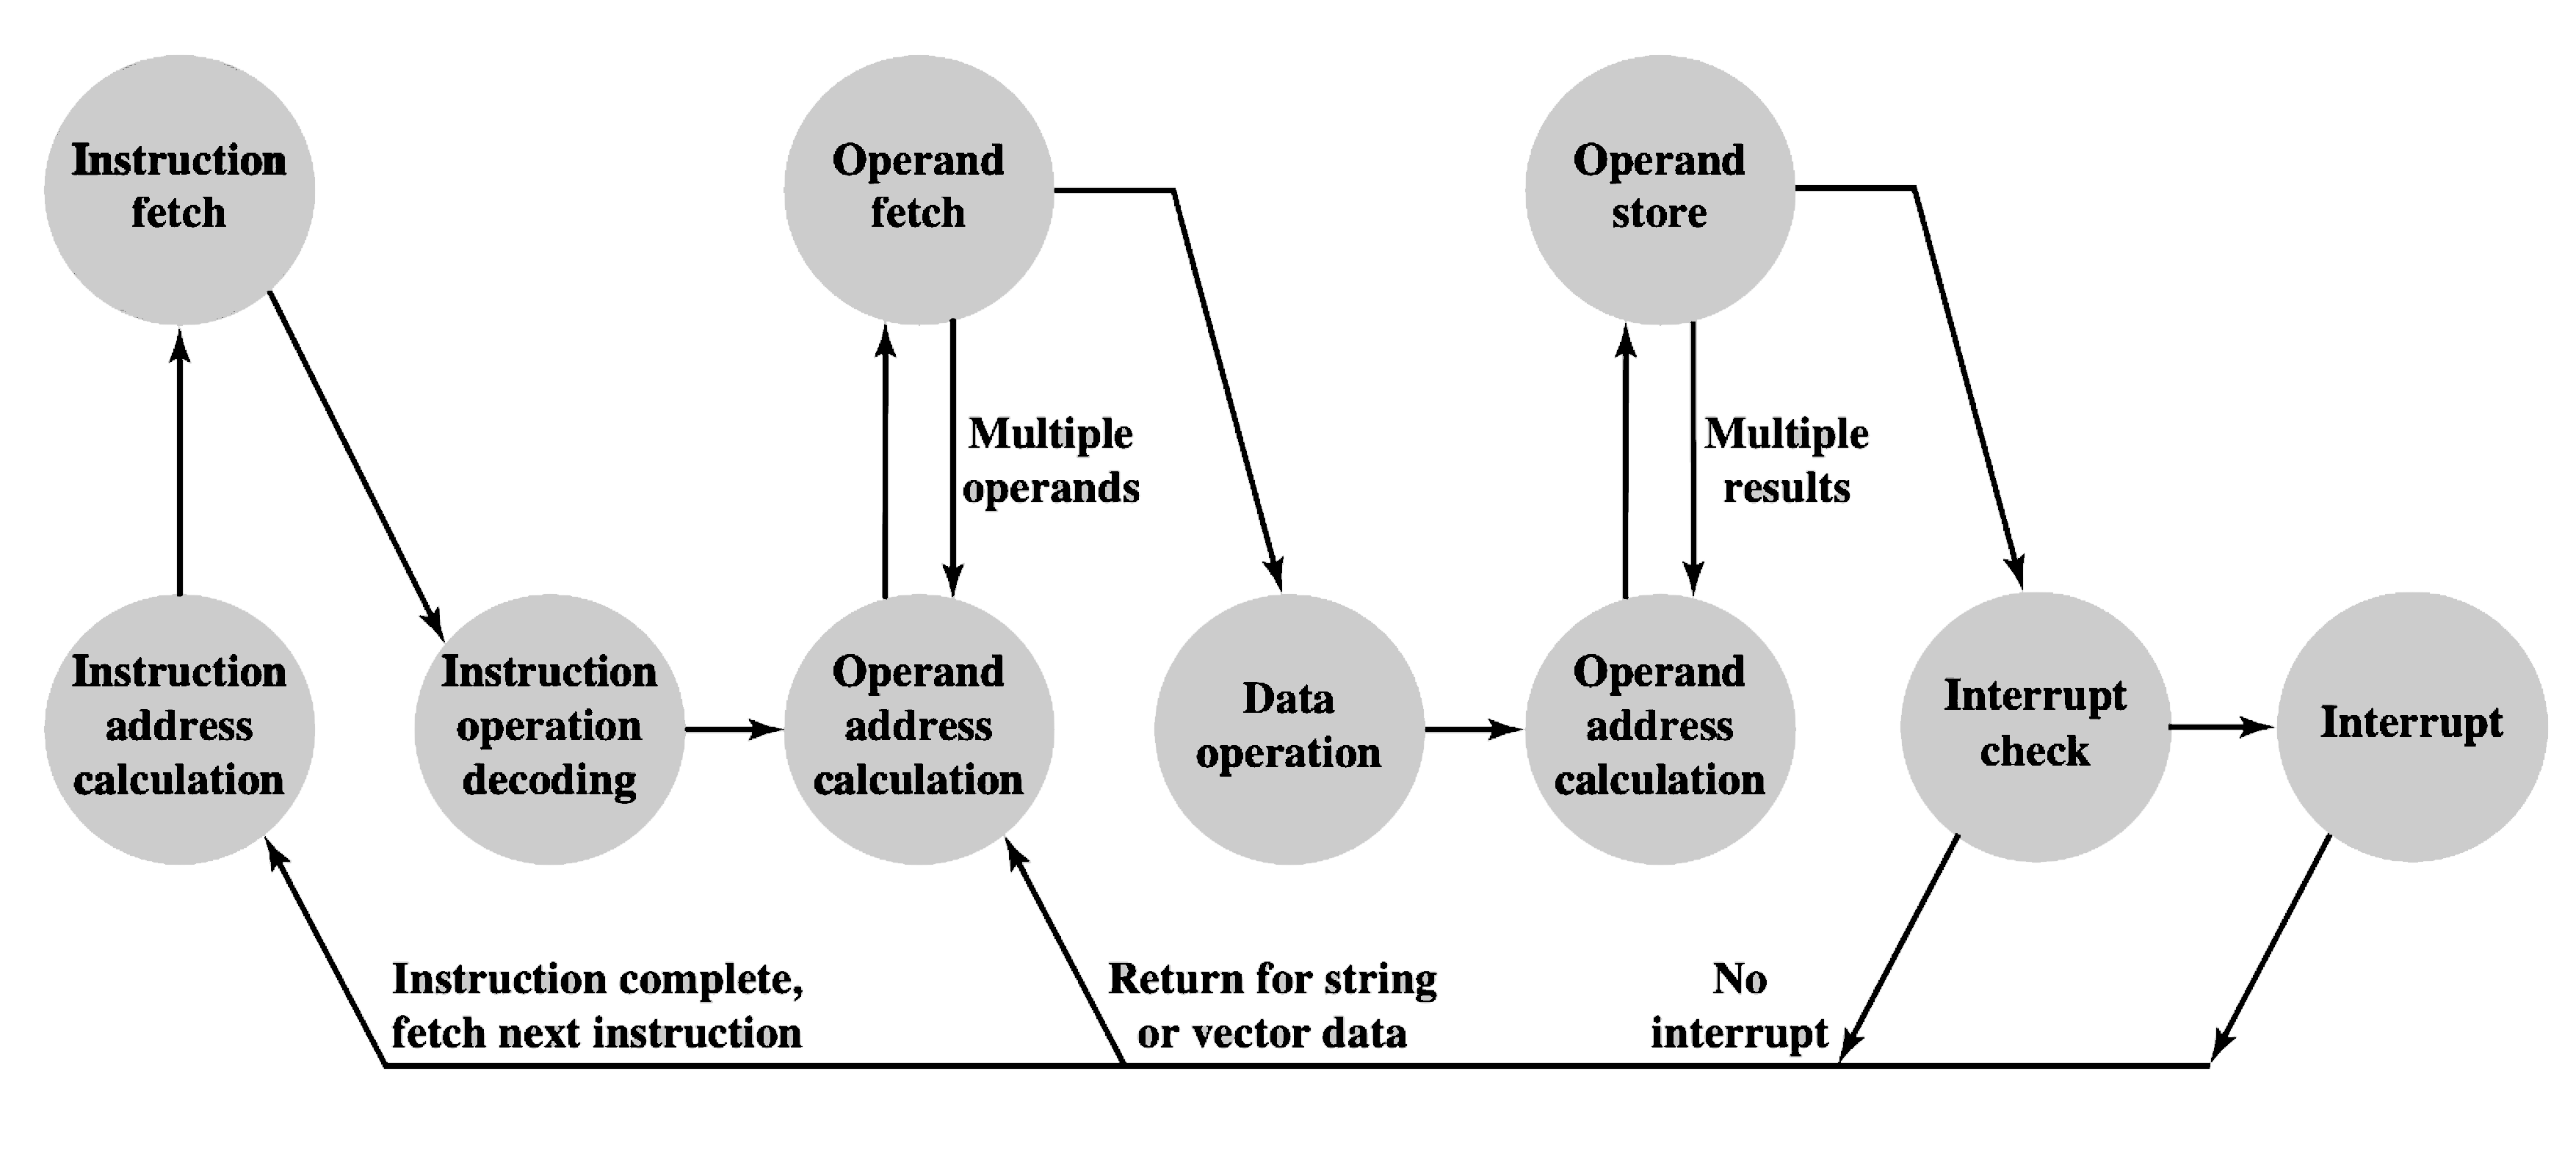
\includegraphics[width=0.4\textwidth]{cycle.png}
    \end{figure}

    % 2023 May
    % Show that AND and NOT gates form a functionally complete set.
    % For the floating-point addition, the first two steps are zero check and significand alignment (making two exponent equal). Next, two significands are added together, there is the possibility of significand overflow. Write down how to deal with this overflow.
    % Explain the relationship between Split Cache and pipeline hazards

    % 2021 May
    % All Solved/Recorded

    % 2020 May
    % Explain why stack pointer is not used in accessing the local variables and function parameters in a stack frame?
    % Show how displacement addressing can be used for this purpose.

    % 2019 May
    % What is the problem with such a long executing instruction?


\end{multicols*}
\end{document}
